\chapter{Perancangan}
\label{chap: perancangan}
	
	Pada bab ini akan dijelaskan mengenai perancangan aplikasi yang dibangun meliputi perancangan kelas, \textit{routes}, \textit{controllers}, \textit{models}, \textit{views}.
	
	\section{Perancangan Kelas}
	\label{sec: rancangKelas}
	
	Seperti yang sudah di jelaskan pada bab sebelumnya, untuk memodelkan sistem penilaian sidang skripsi 2 dengan menggunakan \textit{codeigniter} membutuhkan \textit{routes}, \textit{controllers}, \textit{models}, dan \textit{views}. Hal-hal berikut akan dijelaskan pada subbab selanjutnya.
	
	\section{\textit{Routes}}
	\label{sec: routes}
	
	\textit{Routes} merupakan bagian dari \textit{codeigniter} untuk melakukan pemetaan terhadap lokasi \textit{file controllers} dari aplikasi. Berikut adalah isi dari "config/routes":
	\begin{figure}[H]
		\centering
		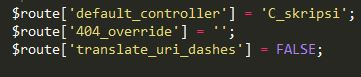
\includegraphics[scale= 1.0]{Gambar/routes}
		\caption {Isi \textit{file routes}}
		\label{fig:routes}
	\end{figure}
	Baris pertama dari kode di atas adalah nama \textit{file controller} yang terletak di \textit{folder controllers} yang akan diambil. Baris kedua merupakan kode untuk menangani \textit{error} yang terjadi jika \textit{file} yang dicari tidak ditemukan, contoh penggunaanya adalah "\$route['404\_override'] = 'errors/page\_missing;". Baris ketiga mempunyai fungsi mengganti seluruh nama \textit{file} yang mengandung '-' menjadi '\_', contoh penggunaanya adalah: "my-controller/index"	menjadi "my\_controller/index".

	\section{\textit{Controllers}}
	\label{sec: controllers}
	
	\textit{Controller} terdiri dari sebuah kelas yang dinamakan "C\_Skripsi". Keseluruhan aktivitas dari sistem informasi penilaian skripsi diatur oleh kelas ini. Berikut adalah gambar kelas diagram dari \textit{controllers}:
	\begin{figure}[H]
		\centering
		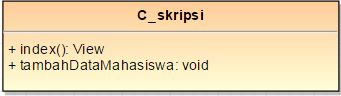
\includegraphics[scale= 1.0]{Gambar/C_skripsi}
		\caption {Gambar diagram kelas \textit{file controllers}}
		\label{fig:controllers}
	\end{figure}
	
	\begin{itemize}
		\item public function index()
		Berfungsi untuk mengarahkan pengguna ke \textit{file views default} dari aplikasi.
		\item public function tambahDataMahasiswa()
		Berfungsi untuk mengambil data dari \textit{view} yang tersedia, untuk kemudian diolah menjadi bahasa sql oleh \textit{models}.
	\end{itemize}
	
	\section{\textit{Models}}
	\label{sec: models}
	
	\textit{Models} mempunyai fungsi menghubungkan \textit{views} dan \textit{controllers} pada \textit{database}. Pada penggunaan \textit{codeigniter}, models dibuat dengan sangat sederhana. Berikut adalah method pada kelas model:
	\begin{figure}[H]
		\centering
		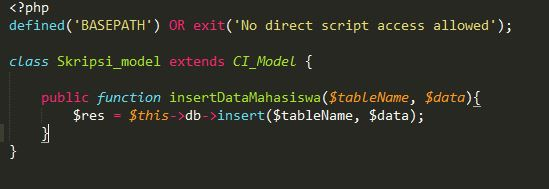
\includegraphics[scale= 1.0]{Gambar/models}
		\caption {Gambar isi dari \textit{file models}}
		\label{fig:models}
	\end{figure}
	\begin{itemize}
		\item public function insertDataMahasiswa(\$tablename, \$data)
		Berfungsi untuk mengolah data yang sudah diolah oleh \textit{controllers} menjadi kueri sql \textit{insert data}.
	\end{itemize}
	
	\section{title}